\section{Time–Frequency Analysis (Q-Transform)} \label{sec:5}

\subsection{Q-Transform}
Time–frequency representation is useful
for visualizing transient gravitational-wave signals. For this purpose,
we use the Q-transform \cite{Chatterji2004,Chatterji2005}.

The Q-transformation is a windowed Fourier transform constructed using
Gaussian-windowed complex sinusoids with constant quality factor \( Q \).
For a strain time series \( h(t) \), it is defined as

\begin{equation}
	X(t_0, f_0) =
	\int_{-\infty}^{\infty}
	h(t)\,
	w_{t_0,f_0,Q}(t)\,
	e^{-2\pi i f_0 t}\, dt ,
\end{equation}

where \( w_{t_0,f_0,Q}(t) \) is a Gaussian window centered at time
\( t_0 \) and frequency \( f_0 \).

The quality factor is given by

\begin{equation}
	Q = \frac{f_0}{\Delta f},
\end{equation}

where \( \Delta f \) is the effective bandwidth. A larger \( Q \)
provides better frequency resolution but poorer time resolution,
while a smaller \( Q \) improves time localization at the expense
of frequency precision.

In gravitational-wave analysis, the Q-transform is commonly applied
to whitened strain data. For compact binary coalescences such as
GW150914, it reveals a characteristic chirp pattern: a signal
that increases in frequency and amplitude with time.

\subsection{Q-Transform Spectrogram}
To visualize the evolution of signal frequency with time, a time--frequency analysis was performed using a Q-transform spectrogram. 

The whitened and bandpass-filtered data in the range 30--300 Hz were used. The analysis window was centered on the merger time and extended $\pm 1$ s.


\begin{figure}[h]
	\centering
	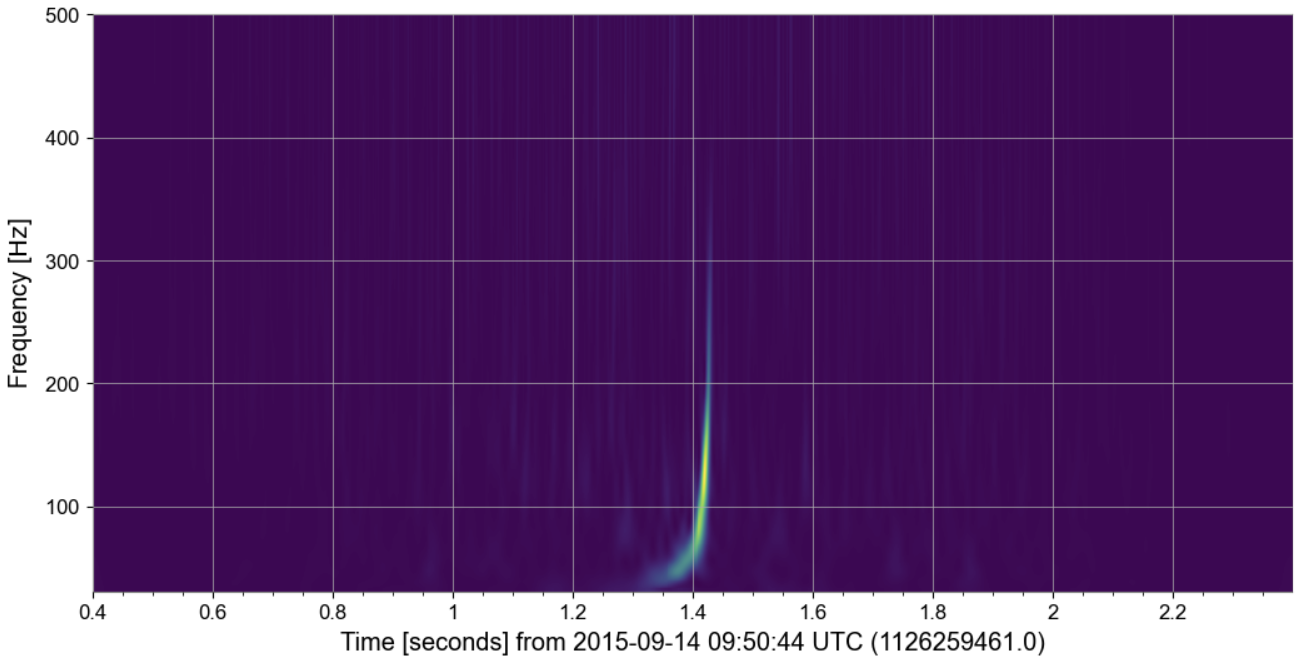
\includegraphics[width=0.9\textwidth]{figure/Qspectrogram}
	\caption{Time--frequency spectrogram of GW150914 showing the characteristic chirp structure.}
	\label{Qtransformation}
\end{figure}


\subsection{Observed Chirp Structure}

The spectrogram reveals a clear upward-sweeping track in frequency over time, characteristic of a compact binary inspiral. The signal begins near $\sim 35$ Hz and increases rapidly in frequency until merger at approximately 150--250 Hz.
The signal duration in the sensitive band is approximately 0.2 s, matching expectations for a high-mass binary system.

\subsection{Off-Source Q-Transformation}
We compute Q-transformation for an off-source window from strain data.
Just like last section our window is 200 s later from the merger time and then compute the Q-transformation.
\begin{figure}[h]
	\centering
	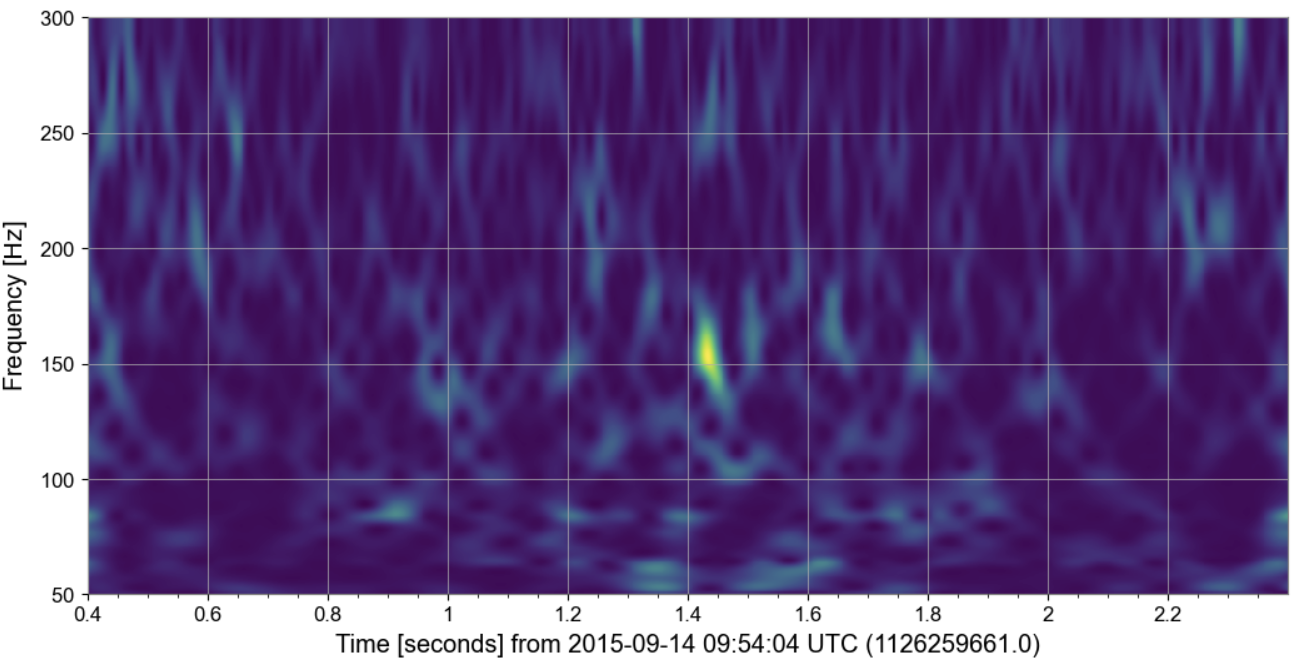
\includegraphics[width=0.9\textwidth]{figure/Qspectrogram_offsource}
	\caption{Off-source Q-transformation, showing no pattern in it.}
	\label{Qtransformation Offsource}
\end{figure}
\subsection{Key Result}

The time--frequency representation clearly demonstrates a monotonic increase in frequency and amplitude consistent with inspiral, merger, and ringdown. The morphology of the chirp provides direct evidence that the source is a compact binary system and is incompatible with stationary or broadband instrumental noise. You can see consistency between whiten data and Q-transformation from fig \ref{filtered data} and \ref{Qtransformation}.
